\documentclass[portrait, final, a0paper, fontscale=0.34]{baposter}
%\documentclass[a4shrink,portrait,final]{baposter}
% Usa a4shrink for an a4 sized paper.

\tracingstats=2

\usepackage[utf8]{inputenc}
\usepackage{calc}
\usepackage{graphicx}
\usepackage{tabularx} % Tables
\usepackage{amsmath}
\usepackage{amssymb}
\usepackage{relsize}
\usepackage{multirow}
\usepackage{rotating}
\usepackage{bm}
\usepackage{url}

% Justify: Left alignment within multicols environment
\usepackage{multicol}
\usepackage{ragged2e} 
\usepackage{etoolbox}
\AtBeginEnvironment{multicols}{\RaggedRight}
% Columns of adjustable size:
\usepackage{vwcol} 

% Fonts
%\usepackage{times}
%\usepackage{helvet}
%\usepackage{bookman}
\usepackage{palatino}

\usetikzlibrary{calc}
\graphicspath{{figures/}}
\DeclareGraphicsExtensions{.pdf,.png,.jpg, .eps}
\newcommand{\captionfont}{\footnotesize}

%%%%%%%%%%%%%%%%%%%%%%%%%%%%%%%%%%%%%%%%%%%%%%%%%%%%%%%%%%%%%%%%%%%%%%%%%%%%%%%%
% Additional (not from the template)
%%%%%%%%%%%%%%%%%%%%%%%%%%%%%%%%%%%%%%%%%%%%%%%%%%%%%%%%%%%%%%%%%%%%%%%%%%%%%%%%
%\usepackage{pgfbaselayers}
%\pgfdeclarelayer{background}
%\pgfdeclarelayer{foreground}
%\pgfsetlayers{background,main,foreground}


%%%%%%%%%%%%%%%%%%%%%%%%%%%%%%%%%%%%%%%%%%%%%%%%%%%%%%%%%%%%%%%%%%%%%%%%%%%%%%%%
% Multicol Settings
%%%%%%%%%%%%%%%%%%%%%%%%%%%%%%%%%%%%%%%%%%%%%%%%%%%%%%%%%%%%%%%%%%%%%%%%%%%%%%%%
\setlength{\columnsep}{1em}
\setlength{\columnseprule}{0mm}


%%%%%%%%%%%%%%%%%%%%%%%%%%%%%%%%%%%%%%%%%%%%%%%%%%%%%%%%%%%%%%%%%%%%%%%%%%%%%%%%
% Save space in lists. Use this after the opening of the list
%%%%%%%%%%%%%%%%%%%%%%%%%%%%%%%%%%%%%%%%%%%%%%%%%%%%%%%%%%%%%%%%%%%%%%%%%%%%%%%%
\newcommand{\compresslist}{%
\setlength{\itemsep}{1pt}%
\setlength{\parskip}{0pt}%
\setlength{\parsep}{0pt}%
}

%%%%%%%%%%%%%%%%%%%%%%%%%%%%%%%%%%%%%%%%%%%%%%%%%%%%%%%%%%%%%%%%%%%%%%%%%%%%%%%%
% Math stuff
%%%%%%%%%%%%%%%%%%%%%%%%%%%%%%%%%%%%%%%%%%%%%%%%%%%%%%%%%%%%%%%%%%%%%%%%%%%%%%%%
\newcommand*\diff{\mathop{}\!\text{d}}
\newcommand*\Diff[1]{\mathop{}\!\text{d^#1}}

%%%%%%%%%%%%%%%%%%%%%%%%%%%%%%%%%%%%%%%%%%%%%%%%%%%%%%%%%%%%%%%%%%%%%%%%%%%%%%
%%% Begin of Document
%%%%%%%%%%%%%%%%%%%%%%%%%%%%%%%%%%%%%%%%%%%%%%%%%%%%%%%%%%%%%%%%%%%%%%%%%%%%%%

\begin{document}

%%%%%%%%%%%%%%%%%%%%%%%%%%%%%%%%%%%%%%%%%%%%%%%%%%%%%%%%%%%%%%%%%%%%%%%%%%%%%%
%%% Here starts the poster
%%%---------------------------------------------------------------------------
%%% Format it to your taste with the options
%%%%%%%%%%%%%%%%%%%%%%%%%%%%%%%%%%%%%%%%%%%%%%%%%%%%%%%%%%%%%%%%%%%%%%%%%%%%%%
% Define some colors
%colors =   [
            %"#08519c",
            %"#9ecae1",
            %"#a63603",
            %"#fdae6b",
            %"#54278f",
            %"#bcbddc",
            %"#006d2c",
            %"#a1d99b"
            %]
\definecolor{bgcolor}{HTML}{FFFFFF}
\definecolor{bgcolor2}{HTML}{FCDFC5}
\definecolor{bordercolor}{HTML}{A63603}
\definecolor{headercolor}{HTML}{FDAE6B}
\definecolor{headerfontcolor}{HTML}{000000}
\definecolor{boxcolor}{HTML}{FFFFFF}

%%
\typeout{Poster Starts}
%\background{
  %\begin{tikzpicture}[remember picture,overlay]%
    %\draw (current page.north west)+(-2em,2em) node[anchor=north west] {\includegraphics[height=1.05\textheight]{drawing.pdf}};
  %\end{tikzpicture}%
%}

\newlength{\leftimgwidth}
\begin{poster}%
  % Poster Options
  {
  % Show grid to help with alignment
  grid=false,
  % Number of columns
  columns=2,
  % Column spacing
  colspacing=1em,
  % Color style
  bgColorOne=bgcolor,
  bgColorTwo=bgcolor2,
  borderColor=bordercolor,
  headerColorOne=headercolor,
  headerColorTwo=white, % only for gradients
  headerFontColor=headerfontcolor,
  boxColorOne=boxcolor,
  boxColorTwo=white,    % only for gradients
  % Format of textbox
  textborder=roundedsmall,
  % Format of text header
  eyecatcher=false,
  headerborder=open, 
  headerheight=0.1\textheight,
  headershape=smallrounded,
  headershade=plain,
  headerfont=\Large\textsf, %Sans Serif
  boxshade=plain,
  background=shadetb,
  %background=user,
  linewidth=2pt
  }
  % Eye Catcher
  {\includegraphics[width=10em]{D1077}} % No eye catcher for this poster. (eyecatcher=no above). If an eye catcher is present, the title is centered between eye-catcher and logo.
  % Title
  {\sf %Sans Serif
  %\bf% Serif
      A Mean Field Theory for a layered \\ Network Model of the Neocortex
\vspace{0.3em}}
  % Authors
  {\sf %Sans Serif
  % Serif
      \vspace{0em}\Large{Friedrich Schuessler\,$^{1}$, Benjamin Merkt\,$^{2}$, Stefan Rotter\,$^{2}$\\
  \normalsize
  $^1$\,Faculty of Physics, University of Freiburg -- 
  $^2$\,Bernstein Center Freiburg and Faculty of Biology, University of Freiburg 
  }
  }
  % University logo
  {% The makebox allows the title to flow into the logo, this is a hack because of the L shaped logo.
    \makebox[8em][r]{%
      \begin{minipage}{16em}
        \hfill
        \includegraphics[height=10em]{unisiegel}
      \end{minipage}
    }
  }

%%%%%%%%%%%%%%%%%%%%%%%%%%%%%%%%%%%%%%%%%%%%%%%%%%%%%%%%%%%%%%%%%%%%%%%%%%%%%%
%%% Now define the boxes that make up the poster
%%%---------------------------------------------------------------------------
%%% Each box has a name and can be placed absolutely or relatively.
%%% The only inconvenience is that you can only specify a relative position 
%%% towards an already declared box. So if you have a box attached to the 
%%% bottom, one to the top and a third one which should be in between, you 
%%% have to specify the top and bottom boxes before you specify the middle 
%%% box.
%%%%%%%%%%%%%%%%%%%%%%%%%%%%%%%%%%%%%%%%%%%%%%%%%%%%%%%%%%%%%%%%%%%%%%%%%%%%%%


%%%%%%%%%%%%%%%%%%%%%%%%%%%%%%%%%%%%%%%%%%%%%%%%%%%%%%%%%%%%%%%%%%%%%%%%%%%%%%
  \headerbox{MOTIVATION}{name=motivation, column=0, span=2}{
%%%%%%%%%%%%%%%%%%%%%%%%%%%%%%%%%%%%%%%%%%%%%%%%%%%%%%%%%%%%%%%%%%%%%%%%%%%%%%
   
\begin{multicols}{2}
In Systems Biology, chemical reaction networks with a high number of species and a low number of observed quantities are very common. In addition, many measurement techniques like quantitative Western blot or protein arrays provide only relative data leading to undetermined scaling parameters in the mathematical model. This results in the problem of structural non-identifiability:  the effect of changing one parameter can be compensated by other parameters.
\end{multicols}
%\vspace{-0.5em}
}


%%%%%%%%%%%%%%%%%%%%%%%%%%%%%%%%%%%%%%%%%%%%%%%%%%%%%%%%%%%%%%%%%%%%%%%%%%%%%%
  \headerbox{SPIKING NETWORK MODEL}{name=network, column=0, span=1, below=motivation}{
%%%%%%%%%%%%%%%%%%%%%%%%%%%%%%%%%%%%%%%%%%%%%%%%%%%%%%%%%%%%%%%%%%%%%%%%%%%%%%
    \centerline{Global network structure}
    \vspace{0.2cm}
    8 populations are arranged in 4 layers, each containing an excitatory and 
    inhibitory population. Neuron and synapse numbers are estimated from 
    experimental data by Potjans and Diesmann. Synapses are drawn randomly until 
    a fixed number is reached. Each neuron receives independent Poissonian 
    spikes as input. Both spike times and membrane potentials are measured. 
    
    \begin{multicols}{3}
        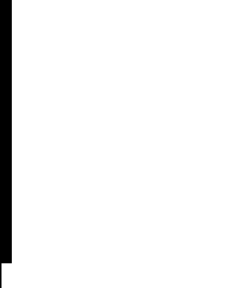
\includegraphics[height=5.0cm]{diagram} 
        \columnbreak

        \includegraphics[height=4.7cm]{population_size} 
        \columnbreak
        
        \includegraphics[height=4.7cm]{synapse_numbers} 
    \end{multicols} 
    %\vspace{0.4cm}

    \centerline{Leaky integrate-and-fire neuron}
    \vspace{0.2cm}
    \begin{vwcol}[widths={0.75, 0.3},
            sep=.4cm, rule=0pt, indent=0em] 
    Membrane potentials $V_i$ are modeled as an RC circuit:
        \begin{equation*}
            \tau_\text{m} \,\frac{\text{d} V_i(t)}{\text{d} t} 
                    = - V_i(t) + \frac{\tau_\text{m}}{C_\text{m}} I_i(t) \,.
        \end{equation*}
        If $V_i(t)$ reaches the threshold $\theta$: \\
        \vspace{0.2cm}
            \quad $\Rightarrow$ 
                Spike is emitted \\
        \vspace{0.2cm}
            \quad $\Rightarrow$ 
                $V_i(t) = V_r$ \,for refractory period $\tau_\text{rp}$ 

    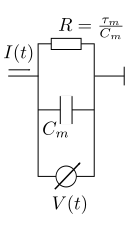
\includegraphics[width=2cm]{RC_circuit}

    \end{vwcol} 

    \vspace{0.5cm}
    \centerline{Current-based synapse model}
    \vspace{0.3cm}
    Each spike elicits a specific current in the postsynaptic neuron:
    \begin{equation*}
    I_{\text{syn}}(t) = w \exp{\left(\frac{-t}{\tau_\text{syn}}\right)}	\,.
    \end{equation*}
    The total incoming current is a sum over all synapses:
    \begin{equation*}
        I_i(t) = 
            \sum_j w_{ij} \sum_k 
            \exp\left(\frac{t - t_j^k - d_{ij}}{\tau_\text{syn}}\right)  \, ,
    \end{equation*}
    where $t^k_j$ is the spike time of the $k$-th spike of neuron $j$.
}


%%%%%%%%%%%%%%%%%%%%%%%%%%%%%%%%%%%%%%%%%%%%%%%%%%%%%%%%%%%%%%%%%%%%%%%%%%%%%%
    \headerbox{MEAN FIELD THEORY}{name=meanfield, column=0, span=1, below=network}{
%%%%%%%%%%%%%%%%%%%%%%%%%%%%%%%%%%%%%%%%%%%%%%%%%%%%%%%%%%%%%%%%%%%%%%%%%%%%%%
    Based on Nicolas Brunel's mean field theory for two populations.
    For a sparsely connected network with uncorrelated input to each neuron, 
    the input current $I_i(t)$ to neuron $i$ in population $a$ can be described by 
    a stochastic equation:
    \begin{align*}
        \frac{\tau_\text{m}}{C_\text{m}} \, I_i(t) &= 
            \mu_a(t) + \sigma_a(t) \sqrt{\tau_\text{m}} \eta_i(t) \\
    \intertext{
    with average part $\mu$ and amplitude $\sigma$
    of the Gaussian white noise $\eta_i$ :
    }
        \mu_a        &= 
            \tau_\text{m}
            \sum_{b \,\in \text{pop.}} C_{ab} \, J_{ab} \, \nu_b +
            \tau_\text{m} C^\text{ext}_a J  \nu_\text{ext} 
            \, ; \\
        {\sigma_a}^2 &= 
            \tau_\text{m} 
            \sum_{b \,\in \text{pop.}} C_{ab} \, {J_{ab}}^2  \, \nu_b + 
            \tau_\text{m} C^\text{ext}_a J^{2} \nu_\text{ext} \,.
    \end{align*}
    Transformation via
    \begin{enumerate}
        \item 
        $\Rightarrow$ Fokker--Planck eq. for membrane potential distributions; 
        \item 
        $\Rightarrow$ Stationary solution to Fokker--Planck eq.;
        \item 
        $\Rightarrow$ Normalization condition for probability distributions;
    \end{enumerate}
    leads to a self-consistency equation for the firing rates $\nu_a$ of each population:
    \begin{equation*}
        \frac{1}{\nu_{a}} = \tau_{rp} 
            + \tau_\text{m} \sqrt{\pi}
                \int_{\frac{V_\text{r} - \mu_{a}}{\sigma_{a}}}^{\frac{\theta - \mu_{a}}{\sigma_{a}}} 
                    e^{u^2} \left(1 + \text{erf}(u)\right) \diff u  
    \end{equation*}
    The equations are coupled via the integral boundaries. Solutions are found
    numerically. 
}


%%%%%%%%%%%%%%%%%%%%%%%%%%%%%%%%%%%%%%%%%%%%%%%%%%%%%%%%%%%%%%%%%%%%%%%%%%%%%%
  \headerbox{RESULTS}{name=results, column=1, span=1, below=motivation}{
%%%%%%%%%%%%%%%%%%%%%%%%%%%%%%%%%%%%%%%%%%%%%%%%%%%%%%%%%%%%%%%%%%%%%%%%%%%%%%
    \includegraphics[height=6cm]{results_rates} 
    
    \includegraphics[height=6cm]{results_membrane} 

    \includegraphics[height=6cm]{simulate_change_g} 

}


%%%%%%%%%%%%%%%%%%%%%%%%%%%%%%%%%%%%%%%%%%%%%%%%%%%%%%%%%%%%%%%%%%%%%%%%%%%%%%
  \headerbox{CONCLUSION}{name=conclusion, column=1, span=1, below=results}{
%%%%%%%%%%%%%%%%%%%%%%%%%%%%%%%%%%%%%%%%%%%%%%%%%%%%%%%%%%%%%%%%%%%%%%%%%%%%%%
\begin{multicols}{2}
    Take home message! 
\end{multicols}
}

%%%%%%%%%%%%%%%%%%%%%%%%%%%%%%%%%%%%%%%%%%%%%%%%%%%%%%%%%%%%%%%%%%%%%%%%%%%%%%
    \headerbox{VARIABLES}{name=variables, column=1, span=1, below=conclusion}{
%%%%%%%%%%%%%%%%%%%%%%%%%%%%%%%%%%%%%%%%%%%%%%%%%%%%%%%%%%%%%%%%%%%%%%%%%%%%%%
\begin{multicols}{2}
\begin{tabular}{>{$}p{1.0cm}<{$} p{4.5cm}}
    \multicolumn{2}{l}{Spiking network model} \\[0.1cm]
    V_i(t)          &  Membrane potential  \\
    \tau_\text{m}   &  Membrane time constant \\ 
    C_\text{m}      &  Membrane capacity  \\
    I_i(t)          &  Input current       \\
    \tau_\text{syn} & Synaptic time constant \\
    w               & Synaptic strength \\
    d               & Delay
\end{tabular} 
\columnbreak

\begin{tabular}{>{$}p{1.0cm}<{$} p{4.5cm}}
    \multicolumn{2}{l}{Mean field model}\\ [0.1cm]
    \multicolumn{2}{l}{Recurrent (populations $a$ and $b$):}\\
    C_{ab}          & Synapse number\\ 
    J_{ab}          & Synaptic weight\\ 
    \nu_a           & Single neuron firing rate\\
    \multicolumn{2}{l}{External:}\\
    C^\text{ext}_{a}& Synapse numbers\\ 
    J               & Synaptic weight *\\ 
    \nu_\text{ext}  & Rate of Poisson process\\[0.15cm]
\end{tabular} 
\end{multicols}
* Synapses are modeled differently: 
Whereas the spiking network model uses current based exponential synapses, 
the mean field theory is originally developed for voltage based delta synapses.
To include the difference, $J$ can be adapted.
}
    

%%%%%%%%%%%%%%%%%%%%%%%%%%%%%%%%%%%%%%%%%%%%%%%%%%%%%%%%%%%%%%%%%%%%%%%%%%%%%%
  \headerbox{REFERENCES}{name=references,column=1,above=bottom}{
%%%%%%%%%%%%%%%%%%%%%%%%%%%%%%%%%%%%%%%%%%%%%%%%%%%%%%%%%%%%%%%%%%%%%%%%%%%%%%
    \smaller
    \bibliographystyle{ieee}
    \renewcommand{\section}[2]{\vskip 0.05em}
      \begin{thebibliography}{1}\itemsep=-0.01em
      \setlength{\baselineskip}{0.4em}
      \bibitem{brunel2000:dynamics}
        N.~Brunel.
        \newblock 
            {D}ynamics of sparsely connected networks of excitatory and inhibitory 
            spiking neurons.
        \newblock 
        \textit{{J}ournal of computational neuroscience}, 2000
      \bibitem{potjans2014:microcircuit}
        T.~Potjans and M.~Diesmann.
        \newblock 
            {T}he cell-type specific cortical microcircuit: {R}elating structure and
            activity in a full-scale spiking network model.
        \newblock 
            \textit{{C}erebral Cortex}, 2014
      \end{thebibliography}
   \vspace{0.3em}
  }


%%%%%%%%%%%%%%%%%%%%%%%%%%%%%%%%%%%%%%%%%%%%%%%%%%%%%%%%%%%%%%%%%%%%%%%%%%%%%%%
  %\headerbox{ACKNOWLEDGEMENTS}{name=acknowledgements,column=1,above=bottom}{
%%%%%%%%%%%%%%%%%%%%%%%%%%%%%%%%%%%%%%%%%%%%%%%%%%%%%%%%%%%%%%%%%%%%%%%%%%%%%%
    %Still?
%}

\end{poster}%
\end{document}
